\documentclass[11pt]{article}

% ---------------------------------------------------------------------------
% Emergence as punctuated collapse of the effective possibility space
% Nature Machine Intelligence Article -- initial submission format
% (flexible format permitted; structure follows Intro/Results/Discussion/
%  Methods with <=3,500 main-text words, 100-150 word abstract, <=6 items).
% ---------------------------------------------------------------------------

\usepackage[a4paper,margin=1in]{geometry}
\usepackage{graphicx}
\usepackage{amsmath,amssymb}
\usepackage{times}
\usepackage[T1]{fontenc}
\usepackage{microtype}
\usepackage{authblk}
\usepackage{setspace}
\usepackage[hidelinks]{hyperref}
\usepackage[numbers,super,sort&compress]{natbib}
\usepackage{caption}
\captionsetup{labelfont=bf,font=small,labelsep=period}
\setlength{\parskip}{0pt}
\linespread{1.25}
\graphicspath{{figures/}}

\renewcommand\Authfont{\normalsize}
\renewcommand\Affilfont{\small\itshape}

\title{\vspace{-1.5em}\bfseries Measuring emergence through collapse of
the effective joint possibility space}

\author[ ]{Author list withheld for double-anonymized review}
\affil[ ]{Affiliations withheld}
\date{}

\begin{document}
\maketitle
\thispagestyle{empty}

% ==========================================================================
\begin{abstract}
\noindent
Emergence is claimed for scaled-model abilities, multi-agent
coordination and collective animal behaviour, yet each field certifies
it with a different instrument, so identical behaviours can be
labelled emergent or not. Here we
define emergence as a spontaneous, persistent, regime-level collapse
of a system's effective joint state--action--trajectory possibility
space, decomposed into environmental, individual, pairwise
and higher-order sources. Calibrated on analytic ground truth and
validated on off-design physics, the instrument shows that
learning populations commit abruptly in every tested system where a
joint exploration barrier---a convention or role with value only once
shared---must be crossed, and smoothly in its absence; that a capability can form smoothly
across training while each deployment of it commits abruptly within
an episode; and that remaining openness predicts, prospectively and
causally in a standard benchmark, whether an intervention can still
change the outcome. Possibility-space collapse turns a contested word
into a measured, falsifiable, actionable quantity.
\end{abstract}

\vspace{0.5em}

% ==========================================================================
\section*{Introduction}

``More is different'' is a claim about organization: many interacting
parts settle into a collective regime none of them specified in
advance\citep{anderson1972more,goldenfeld1999simple,bedau1997weak,holland1998emergence}.
The word \emph{emergence} names that phenomenon in statistical
physics\citep{stanley1971introduction,bak1987self}, in animal
collectives\citep{camazine2001self,couzin2005effective,sumpter2006principles,ballerini2008interaction},
in the new capabilities of scaled neural
networks\citep{wei2022emergent,brown2020language}, and in multi-agent
reinforcement
learning\citep{baker2020emergent,leibo2017multi,jaderberg2019human}.
Yet the fields do not share an instrument: causal-emergence measures
ask whether a coarse-graining has more causal power than its
microstate\citep{hoel2013quantifying,hoel2017map,tononi2016integrated,rosas2020reconciling};
autonomy measures test macro-variable
self-determination\citep{seth2010measuring,barrett2011practical};
partial-information decomposition asks how much of a target is carried
synergistically\citep{williams2010nonnegative,mediano2022greater};
phase-transition theory tracks an order
parameter\citep{strogatz2000kuramoto}; complexity science invokes
irreducibility\citep{crutchfield1994calculi,mitchell2009complexity};
and machine learning reports ``emergent abilities'' as sharp benchmark
upturns against
scale\citep{wei2022emergent,ganguli2022predictability,srivastava2022beyond},
a debate entangled with scaling
laws\citep{kaplan2020scaling,hoffmann2022training} and
grokking\citep{power2022grokking,nanda2023progress}. Each family
evaluates a chosen description---the causal power of a
coarse-graining, the synergy of a target variable, the trajectory of a
hand-picked order parameter; none offers a system-agnostic test for
\emph{when} a collective regime forms, \emph{how abruptly}, and from
\emph{which} interaction structure.

What the fields share is not a measure but an intuition: an emergent
phenomenon is unexpected beforehand yet lawful in
retrospect---surprise has even been proposed as its defining
test\citep{ronald1999design}. But surprise is an observer property,
and a criterion that anything unfamiliar can satisfy names everything
and measures nothing. The formal measures fare little better: some reported emergent
abilities are metric artefacts---change the score function and the
sharp jump disappears\citep{schaeffer2023emergent}. This is the generic risk of
defining emergence on the \emph{observable of convenience}---a
benchmark, an order parameter, a success rate---rather than on the
object that actually reorganizes. Worse, two systems can produce
byte-identical outcomes---identical joint distributions, marginals
and task success---through entirely different couplings (Methods),
and no statistic of that shared distribution can tell them apart.
They become distinguishable only relative to a declared
\emph{observation contract}---which variables are measured, which are
exogenous, which counterfactuals are admissible---under which one can
ask how the effective possibility space closes.

The object is the joint space of what every part \emph{could} still do
together---the effective joint state--action--trajectory space. Before
organization it is wide: an ant colony approaching a gap can still
bridge, cross elsewhere or disperse\citep{reid2015army}. Emergence, on
our account, is the moment this space \emph{collapses} onto a narrow
committed regime---the colony decides, together, to build---and
collapse is not completion: the bridge does not yet exist when the
possibility space has contracted onto building it (Fig.~1). This
definition keeps both halves of the surprise intuition and makes each
measurable: before commitment, low-order observables carry no warning
of what is coming; after it, the collapse has reproducible timing,
sources and consequences. Verdicts are stable within a measured
admissible equivalence class of contracts (Methods).

Here we make three contributions. First, a two-level definition: a
qualification (spontaneous, regime-level, persistent) and a
quantitative \emph{emergence intensity profile} (EIP) whose
axes---amplitude, abruptness, source decomposition---are separately
measured, so abruptness is a phenotype, not a smuggled existence
criterion. Second, a calibrated measurement contract,
matured through preregistered self-falsification, that recovers a
collapse's source on analytic ground truth (72/72 cells) and on
off-design physics. Third, the finding that in \emph{learned} systems
the collapse dissociates cleanly by timescale, varies systematically
with system size and coupling, predicts controllability, and is
\textbf{not} generic: the punctuated form arises spontaneously where
learning must cross a joint exploration barrier, while ordinary
dense-reward optimization collapses smoothly.

% ==========================================================================
\section*{Results}

\subsection*{An operational definition on the right object}

We measure openness as the normalized entropy of the effective joint
possibility distribution, $O_t = H(P_t)/H(P_\mathrm{ref})$, and collapse
as $C_t = 1 - O_t$. Because literal support never shrinks for a
stochastic policy, we work with the \emph{effective} possibility count
$N_\mathrm{eff}=2^{H}$---the formal version of the
$10^n \!\to\! 2^n$ intuition. A system \emph{qualifies} as emergent
when its collapse is regime-level (a structural change in the joint
distribution, not a marginal one), endogenous (generated internally,
declared through a provenance boundary rather than assumed), and
persistent (stable over the declared horizon; recovery and causal
irreversibility are reported separately as robustness properties). Given qualification, we
report an intensity profile rather than a binary label. $P_t$ itself
is defined relative to a declared \emph{observation
contract}---variables, horizon, discretization, reference, provenance
boundary---frozen before any adjudication; objectivity enters through
freezing, measured invariance and refusal outside the contract's
domain (Methods).

The decisive move is the source decomposition. Total collapse splits
along a nested maximum-entropy ladder,
\begin{equation}
C_\mathrm{total} = C_\mathrm{env} + C_\mathrm{individual}
+ C_\mathrm{pair} + C_\mathrm{high},
\end{equation}
so that the interaction cut is a \emph{decomposer}, not a gate, in the
spirit of connected-correlation
expansions\citep{schneidman2003network}. On analytic ground truth with
four independent knobs, each knob moves only its own component, the
ladder is monotone, and hiding an environmental common cause
deterministically re-attributes collapse from $C_\mathrm{env}$ to the
relational channels (five preregistered checks pass;
Extended Data Fig.~1a)---contract-relativity made precise: ``higher-order'' is
defined only relative to what an observer declares exogenous. On a 72-cell factorial (4 sources $\times$ 3
temporal shapes $\times$ 2 stabilities $\times$ 3 magnitudes) the
instrument recovers the source in 72/72 cells, and---the point that
defends against the metric-artefact
critique\citep{schaeffer2023emergent}---amplitude $M$ is invariant
across temporal shape (relative range 0.000) while abruptness $J$
strictly orders punctuated $>$ sigmoid $>$ gradual (Extended Data
Fig.~1b); a
revelation-only or discontinuous-metric control produces exactly zero
collapse.

\subsection*{A breakpoint marks a phenotype, not emergence itself}

Qualification distinguishes emergent from non-emergent organization;
the \emph{breakpoint} distinguishes the punctuated profile from
gradual, non-monotone or unresolved collapse---so a missing
breakpoint never by itself rules emergence out. We fit the
collapse curve with a two-regime model against a one-regime fit by
$\Delta$BIC, inside a saturation-truncated window and behind an
effect-size gate---two amendments forced by preregistered misses and
fixed definitionally on fresh seeds. The matured
detector was frozen and scored on a held-out labelled benchmark: zero
false positives across deceleration, gradual and flat control families
at every tested grid density and noise level, onset power 1.00 at our
operating resolution, and location agreement with a standard
change-point method (Methods). Every headline verdict below is
additionally stable across 243 adjudication contracts (gate, window,
truncation, threshold, grid) and---separately---across a preregistered
battery of representations of the openness object itself; the
measured equivalence class, including the representations that break
it, is reported in Methods.

With the matured detector, an \emph{onset}-type breakpoint (slow $\to$
fast) follows the preregistered profile predictions---present where
the theory predicts punctuated commitment, absent where it predicts
smooth convergence. It appears in a committing ant
colony, in a learned high-order coordination task (7/8 seeds across
original run and five-seed extension), and at the Kuramoto
synchronization
transition\citep{kuramoto1984chemical,strogatz2000kuramoto}. It is
absent---correctly---in an ordinary supervised learner, whose collapse
begins at maximum rate and decelerates (a \emph{knee}, not an onset),
and unresolvable---so not claimed---on stored language-model
checkpoints, whose entropy collapses before the second saved step.

\subsection*{In learned systems, formation and realization dissociate}

The most consequential results are in learned agents, where the
possibility space is shaped by optimization rather than fixed physics.
In a two-phase collective-transport task---sixteen agents must jointly
grip an object before they can push it, structurally delaying the
choice of side---policy-gradient
training\citep{williams1992simple} learns in 10/10 seeds
(success $\geq 0.995$), all with the predicted signature:
side-openness holds at a plateau for $\sim$17--19 steps and then
collapses, with an onset breakpoint in every seed ($\Delta$BIC
45.8--52.7, $t^{*}$ at 16--18; Fig.~2b,d). A preregistered mechanism
control---the same task without the gripping phase---shows no
breakpoint (0/5): it is the structural delay, not learning per se,
that produces punctuated collapse (Fig.~2c). The phenomenon reproduces under a different
algorithm\citep{mnih2016asynchronous} (advantage actor--critic,
byte-identical environment): 5/5 seeds reproduce the
plateau-then-collapse shape and primary hinge ($\Delta$BIC
37.7--45.5)---a partial replication: the strict thinning
clause passes in only 3/5, missing solely on thinned-subsample
detector power.

The same learned system cleanly separates the two senses of emergence
that are usually conflated (Fig.~3). Along the \emph{realization}
axis---within a single episode---collapse is punctuated (5/5
breakpoints). Along the \emph{formation} axis---across training---the
capability appears \emph{smoothly}: outcome-openness expands
(0 $\to$ $\sim$0.65 within $\sim$100 updates) with no structural onset
at either standard or fine 5-update resolution (0/5 on both).
Formation is smooth and expansive; realization is punctuated. This dissociation, in one system with one instrument,
clarifies why debates over whether
scaled-model abilities appear ``suddenly'' have been
inconclusive\citep{wei2022emergent,schaeffer2023emergent}: the
capability may form smoothly while each deployment of it commits
abruptly.

\subsection*{Punctuated collapse arises without designed barriers}

A fair objection is that the grip task's delayed commitment is imposed
by its own state machine---a positive control, not a discovery about
learning. We therefore preregistered two systems in which \emph{no}
environment mechanism delays commitment: every joint regime is
available, and exactly equivalent, from the first update. In a
ten-agent signalling population (five meanings, five symbols, reward
only for successful decoding\citep{lewis1969convention}), any of the
120 codes could be adopted at any moment; yet convention openness
holds at a statistically flat plateau and then collapses with an
onset breakpoint in 4/5 seeds ($\Delta$BIC 17.8--30.1), the breakpoint
($t^{*}=275$--$300$) preceding mutual intelligibility 0.9 (updates
700--1{,}025) in every onset seed, and the five seeds converging to
five \emph{different} codes. A six-agent division-of-labour task
(team reward only when all six interchangeable roles are covered)
shows the same signature more strongly in 5/5 seeds ($\Delta$BIC
53.6--71.7; closing slope $\sim$30$\times$ the plateau slope), again
with collapse preceding capability and five distinct role
permutations. In both
systems the open plateau \emph{is} the joint exploration barrier:
mid-plateau, a probe agent
unilaterally committing to the \emph{best} available code or role
gains essentially nothing (0.011; 0.001); after commitment, the
cheapest unilateral deviation forfeits the structural maximum of the
payoff (0.40 of a 0.40 ceiling; 1.00); and populations from different
seeds are mutually incompatible (cross-seed intelligibility 0.14,
hybrid-team success 0.05, versus $\sim$1.00 within). A code or role
division has value only insofar as others already share it, and the
collapse is nucleated, self-amplifying commitment---the learned
analogue of sharp consensus transitions in naming
games\citep{baronchelli2006sharp,centola2015spontaneous}. Neither
system depends on its tabular parameterization: randomly initialized
neural policies (per-agent MLPs for signalling; one \emph{shared} MLP
for all six role agents) reproduce the signature---onset in 6/7
learned convention seeds and 10/10 role seeds ($\Delta$BIC up to
162), collapse preceding capability in every one, every seed a
different code or permutation. The
neural runs expose a mechanism the theory predicts: random
initialization pre-breaks the symmetry among equivalent regimes,
compressing the plateau roughly tenfold (Methods), and an
initialization-scale sweep moves commitment time in the predicted
direction (monotone for signalling; role-system midpoint non-monotone,
a registered miss). This mechanism---seed
randomness deciding when and where a run commits---matches the
finding that emergent language-model capabilities reflect bimodal
cross-seed distributions rather than deterministic scale
thresholds\citep{zhao2025random}:
each seed crosses the same barrier at a stochastic time, so ensemble
averages blur what single-run collapse curves resolve. Punctuated
collapse is therefore no artefact of designed gates or tabular
parameterization: it arose in every tested system where learning must
cross an endogenous joint-regime barrier, with barrier width set by
how symmetric the competition starts.

\subsection*{The source typology transfers to learned coordination}

Each channel of the ladder is realizable by learning (Fig.~4). A
hidden-coordination task with eight individually-observing agents
produces a purely \emph{relational} collapse: per-agent marginals stay
open (individual entropy $\approx$ 1.0 bit) while total correlation
rises to 6.8/7 bits (Fig.~4a). When the low-order route is blocked with
private information, learning builds a genuinely irreducible
\emph{higher-order} carrier: the textbook XOR structure emerges with
$C_\mathrm{high}$ 0.94--0.96 bits and pairwise $\approx$ 0.0004 bits
throughout the whole formation history (3/3 seeds; Fig.~4b), and
declaring the private cues exogenous re-attributes the identical
collapse to $C_\mathrm{env}$ (Fig.~4c)---the learned version of
contract-relativity. Together these give a sharp statement:
higher-order structure is not unlearnable but
\emph{unfavoured}---gradient learning selects the lowest-order
implementation available and builds irreducible structure only when
information constraints force it\citep{tishby2000information},
echoing difficulties in
emergent-communication\citep{mordatch2018emergence,lazaridou2017multi,foerster2016learning}
and cooperative-MARL\citep{lowe2017multi,sunehag2018value,rashid2018qmix}
studies. Off design, the same ladder correctly reads out Kuramoto
oscillators (uncoupled $\to$ null; common driver $\to$
$C_\mathrm{env}$; single edge $\to$ $C_\mathrm{pair}$), a mechanism
vocabulary it never saw. And at matched task performance, the source
\emph{profile} separates a learned Overcooked
pair\citep{carroll2019utility} from a noise-matched scripted pair
through its environment-conditioned component ($C_\mathrm{env}$
0.0137 [0.0123, 0.0156] vs 0.0005 [0.0004, 0.0007]; Fig.~4d), even
though a single-point coupling measure cannot---the difference is
visible in the collapse composition though in no scalar summary.

\subsection*{Remaining openness predicts controllability}

If emergence is the closing of a possibility space, then how open that
space still is should predict whether the outcome can still be
steered. It does (Fig.~5). In the ant system, per-episode flip-rate
rises strictly with the episode's own remaining openness (0.000 $\to$
0.205 across bins; closed episodes flip 0/2{,}600; flipped episodes
are 0.58 openness units more open, permutation $p < 10^{-4}$ over
8{,}372 paired counterfactuals; Fig.~5d). In the learned grip system,
a counter-regime impulse switches the outcome with probability 1.0 up
to $t=16$ and only 0.27 by $t=30$, and side-openness predicts
switchability with AUC 0.996 (Fig.~5a,b). This is not a time proxy:
at fixed intervention time, openness still separates flippable from
locked episodes (AUC 0.974--0.990 at every tested $\tau$; 20{,}480
episodes per cell). Conditioning additionally on the physical order
parameter removes the signal---the registered boundary: here openness
is an information-sufficient transform of the physical state, and its
value is that it is computable from the policy alone and transfers as
a decision rule. It also works \emph{prospectively}: a rule that waits
until openness first drops to a threshold calibrated on the original
seeds transfers to five unseen seeds, flipping 99.99\% of episodes
while acting 3.8 steps later than the best fixed schedule (99.6\%)
and beating random timing by 21 points---a policy-accessible
intervention coordinate, acting as late as each episode allows. A matched-parameter contrast
isolates the mechanism: when stances are inertial (a hidden
consolidation phase exists), joint openness predicts switchability
\emph{better} than the physical order parameter (AUC 0.886 vs 0.849);
when the single stickiness parameter removes the hidden
phase---all other constants unchanged---the advantage reverses
(0.811 vs 0.884; Fig.~5c). Both orderings were preregistered
predictions. Openness carries controllability
information beyond the order parameter exactly when there is a hidden
regime to consolidate.

\subsection*{Abruptness scales with system size and criticality}

The breakpoint is not specific to learning; it is a systematic feature
of collective self-amplification. In an ant-commitment model a single
chooser \emph{never} shows onset at any gain or grid, while large
colonies always do, and the dependence is quantitative
(Fig.~6a). Because commitment nucleates from binomial fluctuations of
relative size $N^{-1/2}$ that are then amplified at an $N$-independent
rate---a derivation recorded before running---commitment time should
grow logarithmically while the collapse profile stays fixed.
Both predictions hold across $N=1$--$500$: $t_{50}=a+b\ln N$ with
$b=87.6$ (bootstrap 95\% CI [41, 124], $R^{2}=0.93$); the closing width
is $N$-invariant (280--290 trips from $N{=}50$ to $500$); and the
median collapse curves for $N\geq 50$ fall onto a single universal
profile under pure time translation (mean pairwise RMS 0.010 versus
0.266 unaligned; Extended Data Fig.~2)---sharper than
equilibrium-style width
rescaling\citep{stanley1971introduction}. One sub-prediction failed and is reported: at the longer horizon the
onset threshold sits between $N=10$ and $20$, so ``onset at every
$N\geq10$'' was counted a miss. In the Kuramoto system the same instrument tracks the
approach to criticality: across coupling $K=0.9\to2.5$ (10/10 onsets)
the breakpoint time falls monotonically (6.7 $\to$ 1.8) and the
closing slope rises monotonically (0.032 $\to$ 0.199), every
subcritical run is correctly gated null, and the collapse is carried
by the pairwise channel (3/3 seeds;
Fig.~6b)\citep{acebron2005kuramoto}. Abruptness therefore has two
independent, manipulable control parameters---system size and feedback
strength---both preregistered and confirmed.

\subsection*{Where the punctuated form does not appear}

Onset-type collapse is \textbf{not} generic to learned
optimization (Fig.~6c): in standard two-agent Overcooked the learned policies
collapse gradually on both a policy-entropy and a trajectory-occupancy
object (0/3); a registered rescue sequence---smooth consensus, quorum
populations, learning-rate scans---also produced no onset (0/20).

The theory names the missing ingredient---cramped-room geometry pins
the efficient plan, leaving no competing joint regimes---and restoring
it \emph{within the same standard package} restores commitment. In the
official coordination-ring layout, clockwise and counterclockwise
circulation are mirror-equivalent conventions with value only when
shared: with identical PPO mechanics, all eight preregistered
self-play seeds end committed to one direction (final direction
probability 0.97 or 0.03; six counterclockwise, two
clockwise---endogenous symmetry breaking in an unmodified benchmark),
while neither cramped-room control ever commits. The frozen detector
certifies a punctuated onset in one seed (breakpoint at 780k steps
preceding the capability crossing at 1M) and declines the rest: their
formation is non-monotone---commitment forms, dissolves and
re-forms---which the monotone-collapse instrument was not built to
certify, so we count the onset-rate clause as a miss. The regime-level
fact surviving every seed is the committed final convention. A
preregistered within-episode probe locates the commitment level: mid-training episodes drift with a
direction bias but never internally lock (0/5), whereas
final-checkpoint episodes are closed from the first step (initial
openness 0.37, 8/8 seeds; untrained controls stay open, zero false
onsets). The ring convention is a formation-level commitment with no
realization stage---the mechanistic complement of the grip system,
whose commitment lives within the episode.

A final preregistered experiment tests whether this commitment is
causally real. We added unbiased Gaussian noise (two strengths) to
checkpoints taken very early, at the most open point and well after
commitment, then resumed training for 400k steps with byte-identical
mechanics (8 seeds, 48 continuation runs; the seed is the independent
unit). The preregistered primary
endpoint---the perturbation flips or decommits the final
convention---occurs in 7/8 seeds perturbed while open versus 1/8
after commitment (exact paired sign-flip $p=0.016$; run-level 8/16
versus 1/16, Fisher $p=0.008$). Strict direction reversal is
secondary and descriptive (three open-phase flips, zero late;
$p=0.13$ across seeds). Stored openness at the perturbed checkpoint
predicts strict flips (AUC 0.85; descriptive, runs cluster within
seeds), and capability recovers to 0.92 of the unperturbed rate after
late perturbation: what locks is the institution, not the learning. This validates the functional
open-versus-committed distinction, not a causal breakpoint time
(open and late checkpoints also differ in
training time; Methods).

Among classic cases the picture is mixed: Vicsek
flocking\citep{vicsek1995novel}, Swift--Hohenberg pattern
selection\citep{cross1993pattern} and Schelling
segregation\citep{schelling1971dynamic} organize strongly but collapse
\emph{gradually}, while the Potts model\citep{wu1982potts} reproduces
the continuous-versus-first-order distinction through hinge strength
and hysteresis. The result is a classification: collapse profiles sort systems into
punctuated, gradual, parameter-axis and early-warning forms, and onset
appears specifically where a joint-regime barrier---physical (the grip
gate), informational (the blocked low-order channel) or endogenous to
learning (a convention or role with value only once shared)---must be
crossed. Dense-reward optimization with no such barrier collapses
gradually, and our instrument says so.

% ==========================================================================
\section*{Discussion}

We have argued, and measured, that emergence can be defined on the
object that actually reorganizes---the effective joint possibility
space---and that this choice avoids the failure mode behind the
metric-artefact problem\citep{schaeffer2023emergent}: amplitude and
abruptness are provably separate axes, and a discontinuous scoring
function produces zero collapse. The definition
is generative rather than nominal: it supplies a source typology that
transfers from analytic ground truth to physics to learned agents, a
breakpoint whose presence and absence track the theory's predictions,
manipulable dependences of abruptness on size and coupling, and a
control-theoretic payoff: remaining openness predicts whether an
intervention can still flip the outcome.

For machine intelligence specifically, the formation/realization
dissociation clarifies a persistent confusion. ``Emergent abilities'' of
scaled models\citep{wei2022emergent} and the within-run appearance of a
coordinated strategy in self-play
agents\citep{baker2020emergent,vinyals2019grandmaster,bard2020hanabi}
are different events on different timescales: our learned flagship
shows the first as smooth and expansive and the second as punctuated.
Concurrent work detects higher-order structure in multi-agent
language-model groups through partial information
decomposition\citep{riedl2026emergent}; that programme asks whether
synergy is \emph{present}, ours when the joint possibility space
\emph{closes}, how abruptly, through which channel, and whether the
closure can still be steered.

Onset-type
collapse is not generic to deep MARL at current scale: dense-reward
Overcooked optimization collapses gradually. Our designed systems (the
grip gate; the blocked-channel XOR task) are mechanism-isolating
controls, not load-bearing ones: convention formation and role
lock-in reproduce the signature with no designed barrier. What
separates the two classes is a joint
exploration barrier---now directly measured---and the
coordination-ring experiment tests this boundary inside the very
benchmark that produced the negative: restoring competing regimes
restores committed conventions in every seed. Certified onsets remain
rare there because that commitment is non-monotone---an instrument
boundary (Methods); certifying non-monotone commitment and extending to
large-scale self-play are the clear next steps. Three boundaries
remain: the commitment window is not causally verified (a one-pulse
hypothesis failed its falsification clause; formation proved
re-entrant); stored language-model checkpoints are too sparse for any
breakpoint claim; and representation-independence holds as a measured
equivalence class, breaking only where a representation erases the
latent channel; regime-object audits sharpen this
boundary---mis-declared objects lose verdicts, never manufacture them (Methods). Nor is ``emergence $=$ onset breakpoint'' a universal
equivalence: several canonical cases collapse gradually. What we offer
is narrower and more useful---a calibrated, falsifiable instrument
that measures \emph{how}, \emph{when} and \emph{through which channel}
a possibility space closes, and that reports every place it says no. A natural next step is to connect the collapse
object to internal-representation geometry in trained
networks\citep{shai2024transformers}, extending the instrument from
behaviour to mechanism.

% ==========================================================================
\section*{Methods}

\small

\paragraph{Possibility space and openness.}
For a system of $n$ parts we define the effective joint possibility
distribution $P_t$ over the relevant state--action--trajectory support at
analysis time $t$, estimated from rollouts or exact enumeration where
tractable. Openness is $O_t=H(P_t)/H(P_\mathrm{ref})$ with $H$ the
Shannon entropy in bits and $P_\mathrm{ref}$ the maximum-entropy
reference on the same support; collapse is $C_t=1-O_t$ and effective
possibility count is $N_\mathrm{eff}=2^{H(P_t)}$. Entropies are estimated
with a Miller--Madow-style bias correction and, for the joint objects,
with the nested ladder below rather than by direct high-dimensional
estimation.

\paragraph{Intensity profile.}
For a collapse trajectory $C_k$, $k=0,\dots,T$ (entropy reduction from
stage 0, in bits), with peak stage $k_{\mathrm{p}}=\arg\max_k C_k$:
amplitude is $M=C_{k_{\mathrm{p}}}/H(P_\mathrm{ref})$, the peak
reduction as a fraction of the maximum-entropy reference; abruptness is
$J=\max_k \delta_k / \sum_k \delta_k$ over the positive increments
$\delta_k$ of $C_k$ up to the peak---the largest single-stage share of
the total collapse, so $J=1$ for one-step collapse and
$J\approx 1/T$ for uniform gradual collapse; the profile breakpoint
estimate is the stage of the largest increment; and persistence
requires $C_T\geq 0.5\,C_{k_{\mathrm{p}}}$. These are the quantities
calibrated in the 72-cell battery (Extended Data Fig.~1b). One
convention keeps all units consistent: ladder components are raw
entropy reductions in bits and telescope exactly,
$C_\mathrm{env}+C_\mathrm{individual}+C_\mathrm{pair}+C_\mathrm{high}
= H(P_\mathrm{ref})-H(P)$, where the ladder's stage-0 maximum-entropy
distribution is exactly $P_\mathrm{ref}$; the normalized quantities
$O_t$, $C_t$ and $M$ divide by that same reference entropy.

\paragraph{Matched-confound battery.}
Four generators---a central script, a hidden common cause, pure
coincidence and genuine local feedback---are constructed so that no
statistic of the shared joint-action distribution separates them:
joint distributions, single-agent marginals and macroscopic task
outcomes are identical by construction. What separates them is the
declared contract: conditioning on declared exogenous variables,
interaction-severing counterfactuals and persistence checks assign
each generator to its predicted certificate component. Attribution is
therefore contract-relative, not mechanism discovery from outcome
statistics.

\paragraph{Source decomposition.}
The nested maximum-entropy ladder constrains, in order: (i) the
statistics of the declared exogenous variables and conditional
independence given them (environment-conditioned); (ii) additionally
each part's marginal (individual); (iii) additionally all pairwise
marginals, following the connected-correlation construction of
Schneidman et al.\citep{schneidman2003network} (pairwise); and (iv) the
full joint. $C_\mathrm{env}$, $C_\mathrm{individual}$,
$C_\mathrm{pair}$ and $C_\mathrm{high}$ are the successive entropy
reductions. Three properties matter for interpretation. First, each
stage only adds constraints, so entropy is non-increasing along the
ladder and every component is non-negative by construction. Second,
the ladder is a sequence of information projections defined for
\emph{every} joint distribution---it is not a parametric model of the
data---so ``model misspecification'' does not arise; a generator that
mixes sources simply deposits entropy reduction at several levels at
once, which is the intended reading. Third, the stage order is not a
free knob: given a declared exogeneity boundary, the
individual-to-pairwise-to-higher progression is the canonical hierarchy
of marginal constraints, and the only genuinely movable choice---the
boundary itself---is exactly the declared contract-relativity
demonstrated in Fig.~4c. The provenance boundary is fixed before
analysis in every experiment. A preregistered stress audit quantifies
the remaining freedoms. Off-family generators the ladder was never
built from are attributed correctly (a modular-sum triple with exactly
independent pairwise marginals loads 3.32 bits on $C_\mathrm{high}$
with $C_\mathrm{pair}=0$; a Markov copy chain loads purely on
$C_\mathrm{pair}$ with $C_\mathrm{high}=0$; fifty random Dirichlet
joints give zero negative components and an exact telescoping
identity). The constraint sets form a filtration, so no
individual/environment reordering exists; the one genuine order
freedom---declaring the environment before or after the pairwise
stage---leaves the individual and higher-order components exactly
invariant and moves the environment/pairwise split by at most 0.26
bits across an 81-cell grid. Finite-sample behaviour is measured, not
assumed: median absolute component error is $\leq$0.018 bits at
$3\times10^{4}$ samples for the three-agent test system, with no
negative estimates in 120 runs, and the small-sample bias concentrates
in $C_\mathrm{high}$ (0.31 bits at $n=300$), which sets an explicit
sample floor for higher-order claims. One registered audit prediction
missed: when generator knobs interact strongly (pairwise copying under
a parity mechanism), realized structure genuinely relocates across
orders---copying makes the parity constraint first-order---so the
ladder attributes it to the individual level. We report this as a
property, not a defect: the ladder measures realized distributional
structure, not generator labels.

\paragraph{Breakpoint detector.}
Collapse curves are fit with one- and two-regime piecewise-linear models;
the breakpoint is accepted when the two-regime $\Delta$BIC exceeds 10 and
survives parity-thinning of the checkpoint grid, the curve passes an
effect-size gate (max drop $\geq 0.1$), and the analysis window is
truncated at saturation (first point within 5\% of the final value). An
\emph{onset} type requires
$|\mathrm{slope}_\mathrm{after}| > |\mathrm{slope}_\mathrm{before}|$; the
reverse ordering is a \emph{deceleration} knee. The gate and
saturation-truncation were added in response to two preregistered control
failures (a flat subcritical false positive; a saturation-knee capture)
and re-tested on fresh seeds.

\paragraph{Detector validation.}
Because the detector was matured through its own registered failures, it
was frozen and then scored on an independent, preregistered synthetic
benchmark of 200 curves per family (onset, deceleration knee, linear
gradual, sigmoid, flat) per condition, with labels fixed before running.
At the reference operating point (80 grid points, noise
$\sigma=0.02$) onset power is 1.00 and the false-positive rate across
all control families is 0.000; power rises monotonically with grid
density (0.00/0.62/0.995/1.00 at 12/20/40/80 points) while the
false-positive rate remains 0.000 at every density, and degrades
gracefully with noise (0.93 at $\sigma=0.08$, false positives 0.000
throughout; Supplementary Table~1). Zero observed false positives among 200 curves per control
family bounds the true rate at $\leq$0.5\% per condition (95\%
rule-of-three over the pooled 600 controls); we report the bound rather
than claiming the rate is exactly zero. The detector adjudicates
monotone collapse only: a preregistered extension to non-monotone
commitment (a settled-openness envelope recording irrevocable closure)
kept false positives below 0.05 in every validation round but never
exceeded 0.71 power against its required 0.90 on synthetic
non-monotone positives, and under its own preregistered stopping rule
was closed without ever being applied to system data; certifying
non-monotone regime formation therefore remains an open instrument
problem, which is why the coordination-ring onset count is reported at
1/8. A semi-synthetic injection audit quantifies the matching noise
floor: commitments injected at known times into the ring pipeline's
own estimator (real grids, real committed-episode counts, binomial
direction noise) are recovered with false-positive rate 0.01 and
median $t^{*}$ error 1\% of span, but detection power saturates at
0.88 (registered threshold 0.90, recorded as a near-miss)---the
30-episode evaluation budget itself caps single-curve power below the
synthetic-library ceiling. Breakpoint locations agree with an independent standard
change-point method (binary segmentation, RBF cost) to within 10\% of
span on onset curves; unlike generic change-point detection, the
instrument correctly declines to call onset on deceleration and gradual
curves. The zero power at 12 grid points sets the resolution floor:
it is why no claim is made on sparse language-model checkpoint grids.

\paragraph{Adjudication-contract robustness.}
All headline breakpoint verdicts were re-adjudicated across 243 analysis
contracts per system, crossing saturation fraction
$\{0.02,0.05,0.1\}$, analysis window $\{0.75,0.875,1.0\}$ of the curve,
effect-size gate $\{0.05,0.1,0.15\}$, $\Delta$BIC threshold
$\{8,10,12\}$ and checkpoint-grid stride $\{1,2,3\}$. For the grip
flagship, the committing ant colony and the learned high-order task the
onset verdict is unchanged in 100\% of adequate-resolution cells and the
breakpoint location varies by 1\%, 8\% and 11\% of curve span
respectively; aggressive grid coarsening reduces detectability (a power
effect quantified by the validation benchmark above), never the
location (Supplementary Table~2). The collapse object itself is fixed by the theory (the joint
commitment space), not chosen by fit: the raw action-entropy of the grip
system \emph{rises} during the same window and is reported as such.

\paragraph{Observation contract.}
Every entropy is computed relative to a declared contract with six
components: the variables admitted to the joint space, the trajectory
horizon, the discretization, the reference distribution (maximum
entropy on the same support), the probability-truncation rule, and the
provenance boundary separating environment from system. Two properties
anchor the contract's objectivity. First, an invariance that holds
exactly: $O_t$ is unchanged under any bijective recoding of states or
actions, because Shannon entropy is permutation-invariant and the
reference is defined on the same support---openness cannot be
manufactured or destroyed by renaming. Second, an admissible class
that is measured rather than assumed: representations remain
admissible while they separate the competing regimes at or above the
detector's resolution floor, and the equivalence battery below maps
where that class ends (non-injective coarse-graining that merges
regime-distinguishing states, or truncation that deletes the latent
channel, breaks the verdict---mechanistically, not capriciously). The
contract is frozen before adjudication and the instrument refuses
outside it. One component deserves emphasis: the framework does not
discover the regime variable from raw trajectories; it certifies a
\emph{declared} regime object. In every system here that object was
named before analysis with a domain justification---side choice
(bridge), grip configuration and push side (transport), code mapping
(signalling), role permutation (division of labour), XOR carrier
(blocked channel), circulation direction (Overcooked ring), phase
locking (Kuramoto), magnetization sector (Potts)---and where no
credible regime object exists the correct output is refusal, not a
verdict. The instrument is thus a general measurement contract for
declared collective regime objects, not an automatic emergence
detector for arbitrary raw systems. The analyst's freedom is thereby
the same freedom every measurement has---the choice of ensemble in
thermodynamics, of coordinates in mechanics---made explicit, fixed in
advance, and accompanied by its measured range of validity.

\paragraph{Representation equivalence.}
Detector settings and measurement representations are different
freedoms, so they were audited separately. On byte-identical retrained
seeds we recomputed the openness object under twelve preregistered
representations---for the convention system, the population-mean
mapping, per-agent mean entropy, the listener-side dual, a
2{,}048-sample behavioural estimate, a checkpoint-zero empirical
reference, $\varepsilon=0.01$ truncation and 5$\to$3 symbol
coarse-graining; for the grip system, policy probabilities, state
quantization at 0.1 and at 0.5, realized 16-agent action counts, and
$\varepsilon=0.01$ truncation---and adjudicated each with the frozen
detector. The onset verdict survives in 8/12 cells and the breakpoint
location is essentially representation-invariant wherever a verdict
exists: $t^{*}=250$--$300$ of a 4{,}000-update span (1.25\%) in the
convention system, and identical ($t^{*}=17$) in every preserving grip
representation. The registered $\geq$90\% preservation bar was missed,
so per the registered clause we report the measured equivalence class
instead of claiming blanket invariance. All four breaking cells fail
for identifiable reasons and still locate the commitment at
$t\approx19$--$22$: two fall just below the conservative
$\Delta$BIC$=10$ bar while agreeing on location (per-agent entropy,
which is an individual-level object rather than the joint convention;
5$\to$3 binning); 0.5-level state quantization compresses the
transition into a one-to-two-checkpoint cliff that fails the frozen
thinning clause (a resolution limit, not a disappearance: the unthinned
fit gives $\Delta$BIC 111, onset-type); and $\varepsilon$-truncation
zeroes the side channel while it is latent ($<$1\% of action mass
during the grip phase), making the object non-monotone---truncating
small probabilities destroys precisely the still-open possibilities the
object exists to measure. The equivalence class is therefore:
verdict and location survive object dualities, behavioural sampling,
reference changes and state coarse-graining down to the detector's
resolution floor; they break only when the representation erases the
latent channel or compresses the transition below that floor
(Supplementary Table~3).

\paragraph{Regime-object audits.}
The declared regime object is an analyst choice, so two further
preregistered audits test whether verdicts depend on it. An
\emph{ensemble} audit enumerates, from each environment specification
alone, the alternative regime variables an independent analyst could
plausibly have declared (convention: the listener code, the composed
speaker--listener channel, a single-meaning sub-regime; roles: one
agent's role, one role's owner; grip: the realized force direction),
together with control variables that erase the symmetric competition
or are exogenous by construction, and adjudicates every candidate with
the frozen detector on byte-identical reruns. On the formation axis,
admissible alternatives reproduce the declared verdict in 22/25 cells
(roles 10/10, listener code 5/5) and every co-certified breakpoint
falls within the detector's span tolerance (19/19); the disagreements
are one sub-regime cell below the evidence threshold and the composed
channel in two seeds---a two-stage regime whose late second collapse
the monotone detector declines. None of the 20 control cells certifies
an onset. A \emph{discovery} audit removes the analyst: one fixed
recipe (k-means on raw episode records, $k$ by silhouette, no
per-system tuning) defines regime variables from behaviour alone. On
the formation axis it reproduces 6/10 verdicts, with both convention
disagreements at the detector threshold ($\Delta$BIC 6.9 and 9.8
against 10) and one roles cell failing only the thinning clause; on
the realization axis, state-trace and windowed-force proxies qualify
the collapse but miss the strict onset bar in all three registered
constructions (best $\Delta$BIC 12.6), and untrained grip controls
certify onset because the structural gate delays commitment for any
policy---the mechanism control's own prediction. The registered
agreement targets were missed (ensemble 22/30 against 24/30; discovery
6/15 against 12/15) and are reported with this diagnosis. Across all
105 audit cells the failures are one-directional: mis-declared or
lower-power regime objects lose verdicts, and exactly one gains one
(the event-level convention variable in the seed whose declared object
shows no onset, $\Delta$BIC 23.6). The declaration is a power
parameter, not a cherry-picking lever (Supplementary Tables~4
and~5).

\paragraph{Emergence certificate.}
The frozen instruments are packaged into a single standardized
adjudication script (\texttt{emergence\_\allowbreak certificate.py})
so that a new system
receives a reproducible verdict: a three-condition qualification
(regime-level: the collapse gate \emph{and}, where the source analysis
is available, joint-beyond-marginal reorganization; endogenous: the
declared provenance boundary; persistent: no re-opening beyond 0.1 of
reference within the observed window), the intensity profile as a
vector (amplitude, abruptness class, sharpness, $t^{*}$, source
ranking), and a categorical verdict with an explicit
\emph{unresolvable} class below the measured power floor and a
low-power flag between 12 and 40 grid points. We deliberately do not
output a scalar ``emergence score'': amplitude and abruptness are
demonstrated independent axes, and any fixed weighting of them would
reintroduce the observable-of-convenience failure this framework
exists to remove. Applied to the paper's systems, the certificate
issues ``emergent: punctuated'' for the grip, convention, role and
$N{=}100$ ant systems; the single-ant control---with nearly the same
amplitude (0.92) as the colony---correctly \emph{fails} qualification,
because its collapse is purely individual-source rather than a joint
regime, and the Overcooked occupancy object falls below the collapse
gate with a low-power flag. Same entropy drop, different verdicts: the
discrimination is exactly what a bare entropy measure cannot provide
(per-system qualification table in Supplementary Table~6).

\paragraph{Learned systems.}
The grip-transport flagship uses 16 agents, grip threshold 6, a two-phase
grip-then-push dynamics (grip gain 0.06, decay 0.01), trained by
REINFORCE\citep{williams1992simple} (1{,}200 updates, batch 512, learning
rate $2\times10^{-3}$) and, for the robustness check, by advantage
actor--critic\citep{mnih2016asynchronous} on identical environment
parameters (per-seed statistics in Supplementary Table~7). The hidden-coordination flagship uses 8 individually-observing
agents with per-agent stances; the sticky variant sets stance-change
probability 0.25 and the matched control sets it to 1.0 with all other
constants imported unchanged. Overcooked runs use the standard
cramped-room layout\citep{carroll2019utility}. The non-constructed
convention system is a ten-agent Lewis signalling
population\citep{lewis1969convention} (five meanings, five symbols,
tabular policies, REINFORCE, 512 random speaker--listener pairs per
update, 4{,}000 updates); the role system is six agents choosing among
six roles with team reward only for full coverage (6{,}000 updates,
otherwise identical training); in both, openness is computed from
policy probabilities at 25-update checkpoints and adjudicated by the
frozen detector (Supplementary Table~8). The neural replications keep both environments and
recipes fixed and replace the tables with one-hidden-layer networks
(32 tanh units, Adam $3\times10^{-3}$, ten fresh seeds per system):
per-agent speaker and listener MLPs for the signalling population, and
a single MLP shared by all six role agents, so that role
differentiation must emerge inside one network. Because random
initialization compresses commitment into the first few hundred
updates, the neural runs are evaluated at 5-update resolution---a
preregistered measurement-density amendment justified by the
detector's validated grid-power curve; at the original 25-update grid
the onsets are under-resolved (1/7 and 1/10), which is recorded
alongside the fine-grid result (Supplementary Table~9). The initialization sweep varies the
input-weight scale $\sigma\in\{0.02,0.1,0.45\}$ at five seeds per
cell. The coordination-ring study trains standard
\texttt{overcooked\_ai} self-play PPO (mechanics and budget identical
to the cramped-room runs, 2M steps) on the official
\texttt{coordination\_ring} layout, eight seeds, checkpoints every 20k
steps; the regime object is the entropy of the pair's circulation
direction (net winding around the central counter, Laplace-smoothed
over 30 evaluation episodes per checkpoint), declared before running
(per-seed conventions in Supplementary Table~10).
A parallel preregistered attempt on the unmodified MPE
\texttt{simple\_spread} benchmark did not reach its frozen competence
precondition (conflict-episode coverage 3\% after 3{,}000 PPO updates)
and is recorded as a training failure with no theory claim made either
way. The causal commitment test perturbs stored ring checkpoints at
100k steps, at the seed's most-open checkpoint (last with direction
probability in $[0.3,0.7]$ and $\geq 20$ committed evaluation
episodes), and at 1.6M steps, adding per-tensor Gaussian noise of 0.25
or 0.5 relative standard deviations, resuming training for exactly
400k steps with unchanged mechanics and schedule position, and scoring
the final convention against the seed's unperturbed direction; all
times, scales, margins and clauses were frozen in the protocol file
before any run. Because the two noise scales share a training seed,
continuation runs cluster within seeds; the run-level Fisher test was
the frozen clause, and a stricter seed-level paired analysis (exact
sign-flip permutation over the eight seeds, labeled post-hoc in the
protocol file) confirms the primary endpoint and demotes the strict
direction-reversal contrast to descriptive. Because open and late
checkpoints differ in training time as well as openness, the timing
contrast alone cannot exclude generic training maturity; the
fixed-time analysis that rules out the time confound exists in the
grip system and has not yet been run here. The finite-size study uses sizes
$N\in\{1,2,5,10,20,50,100,200,500\}$, 30 episodes per size and a
1{,}500-trip horizon, with $t_{50}$ and width read from median
openness crossings and the log-law slope bootstrapped over episodes
(Supplementary Table~11).
The ant, Kuramoto, Potts, Vicsek, Swift--Hohenberg and Schelling models
follow their standard definitions (Supplementary Methods).

\paragraph{Barrier measurement.}
The joint-exploration-barrier claim is tested by deterministic replay
of both learned positive systems with policy snapshots at every
checkpoint (replay validity: all ten re-run seeds reproduce the stored
final codes and role assignments exactly). At the checkpoint nearest
$t^{*}/2$ (onset seeds only), the unilateral adoption gain of agent
$i$ is the payoff of a probe hard-committed to the best of all $K!$
codes (respectively all $R$ role locks) against the unmodified
population, minus the payoff of $i$'s own current policy, averaged
over agents; payoff is symmetric expected intelligibility with a
random partner (convention) or the permanent of the row-stochastic
role matrix (roles). At the final checkpoint the unilateral deviation
cost is the payoff on the population's majority regime minus the best
payoff over all alternative committed regimes. Cross-play pairs
speaker populations with listener populations from different seeds
(20 ordered pairs) and assembles hybrid role teams from every proper
subset split of every distinct-assignment seed pair (620 teams). All
four outcome clauses were frozen before the run; one
threshold-calibration miss (the convention deviation-cost clause set
0.50 where the payoff structure caps the cost at
$0.4\times$within-population payoff for $K{=}5$ permutation codes,
the measured value 0.3996 sitting at that ceiling) is reported
verbatim in the protocol file. What these quantities measure is a
\emph{unilateral coordination barrier}---the absence of single-agent
payoff gradient toward any regime, and the single-agent cost of
leaving one---not the full performance landscape over joint policy
paths; multi-agent coordinated escape routes are not enumerated.

\paragraph{Scalability.}
The pipeline's cost is dominated by openness estimation, not by the
detector (which fits two linear models per gridpoint and is linear in
grid length). Openness requires the entropy of the declared
possibility object, estimated either exactly from policy
probabilities (learned tabular and neural systems), or from empirical
distributions over the declared coarse-graining (physical systems),
whose sample complexity we measured directly: in the finite-sample
audit the median absolute error of every ladder component is
$\leq$0.02 bits at $3\times10^{4}$ samples, rising at 300 samples to
0.09 bits (individual), 0.31 (higher-order) and 0.81 (pairwise), so
the pairwise term is the first casualty of scarce data. Total
openness itself is linear in population size times horizon, and the
breakpoint stage ran unchanged at population sizes up to $N{=}500$ in
the finite-size study; the source decomposition is the only
superlinear stage (pairwise marginals cost $O(N^{2})$ and the
higher-order maximum-entropy fit is the practical ceiling), so
qualification and profile can always be computed at scales where the
full typology cannot. All experiments in this paper run on CPU except
the Overcooked PPO training; no single run exceeds a day of
wall-clock time.

\paragraph{Preregistration and integrity.}
Every predicted outcome was frozen, with an explicit falsification
clause, in an internal protocol file before the corresponding run;
passes and misses are reported identically, and each amendment is
recorded in place with its trigger (the complete ledger is collected
in Supplementary Note~1). We characterize these as
internally time-stamped frozen protocols rather than third-party
registrations: they were not lodged with an external registry, and we
release them verbatim---including every miss, every failed instrument
extension and every post-hoc analysis labeled as such---together with
the code, raw outputs and an output manifest, so that the ordering of
protocol and result can be audited from the released record. All
numbers in the main text and figures are produced by a single
extraction script run directly against the raw output files; no value
is transcribed by hand. One float32 numerical defect (an entropy clamp
that rounded to a degenerate value) was found, fixed in code, and both
affected experiments were rerun with identical seeds, with the
corrupted outputs archived. No thresholds were changed after seeing
results.

\paragraph{Reporting summary.}
Further information on research design is available in the Nature
Portfolio Reporting Summary linked to this article. The use of
large-language-model agents is disclosed in the dedicated section in
the back matter.

\normalsize

\section*{Data availability}
\small
The raw output of every experiment (one JSON file per registered run),
together with the frozen protocol files that fix each prediction and
falsification clause before running, is provided in the accompanying
repository and will be archived with a permanent DOI on Zenodo upon
acceptance. Source data for
each main-text figure are generated directly from these files by the
plotting script; no intermediate hand-edited data are used.
\normalsize

\section*{Code availability}
\small
All simulation, training, analysis and figure-generation code is
available in the accompanying repository and will be archived on
Zenodo upon acceptance. The
manuscript's quantitative claims are reproduced by a single extraction
script (\texttt{manuscript\_numbers.py}) that reads the raw outputs and
prints every number cited in the text and figures, by a
figure-generation script (\texttt{make\_figures.py}) that draws all
panels from the same files, and by \texttt{make\_si\_tables.py}, which
generates every Supplementary Table directly from the raw outputs.
\normalsize

\section*{Acknowledgements}
\small
Acknowledgements withheld for double-anonymized review.
\normalsize

\section*{Author contributions}
\small
Author contributions withheld for double-anonymized review.
\normalsize

\section*{Competing interests}
\small
The authors declare no competing interests.
\normalsize

\section*{Use of large language models}
\small
Large language models were used, under the authors' direction and
continuous review, to assist in writing and debugging code and in
drafting and editing text. The experimental designs, protocols and
adjudication criteria were specified by the authors, who reviewed and
validated all code, protocols and analyses and take full
responsibility for all claims.
\normalsize

% ==========================================================================
\clearpage
\bibliographystyle{unsrtnat}
\bibliography{references}

% ==========================================================================
\clearpage

\begin{figure}[p]
\centering
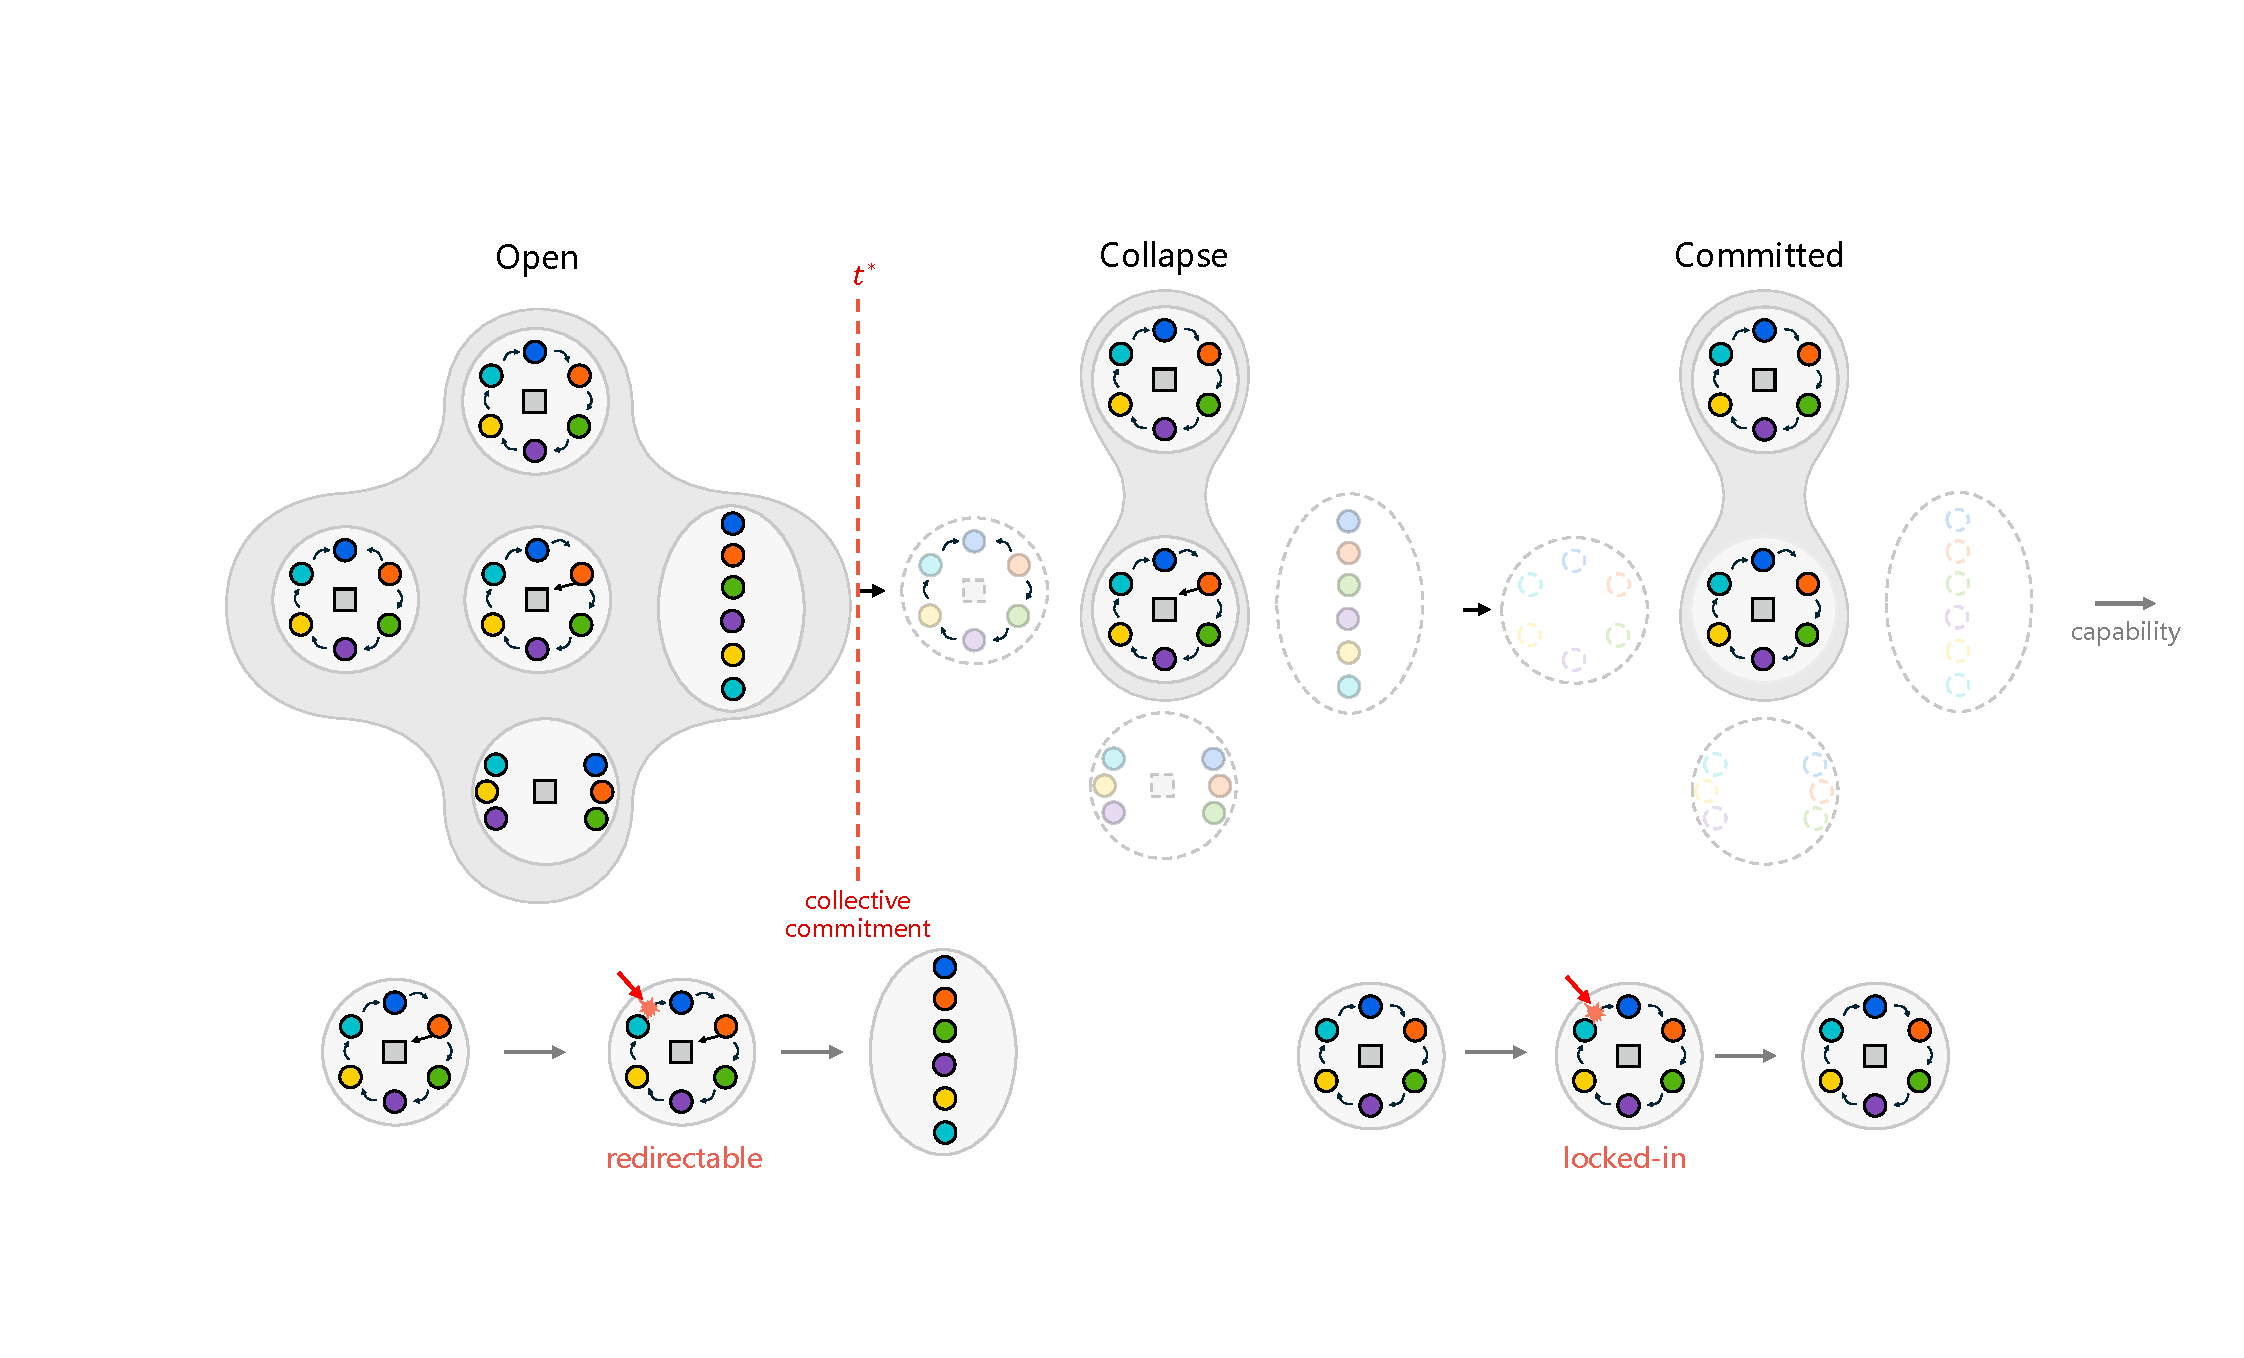
\includegraphics[width=\textwidth]{fig0_overview.pdf}
\caption{\textbf{Emergence as possibility collapse.}
A population of learning agents (coloured dots) starts with many joint
futures open (grey): several collective regimes---here a ring and a
line---are still reachable. At a breakpoint $t^{*}$ the joint
possibility space begins to contract; alternatives fade until the
population is committed to a single regime, and only after this
collective commitment does the capability appear. Bottom, the
practical consequence: while the space is open, a small perturbation
(red arrow) can still redirect the population to a different regime;
after commitment the same perturbation changes nothing---the regime is
locked in.}
\end{figure}

\begin{figure}[t]
\centering
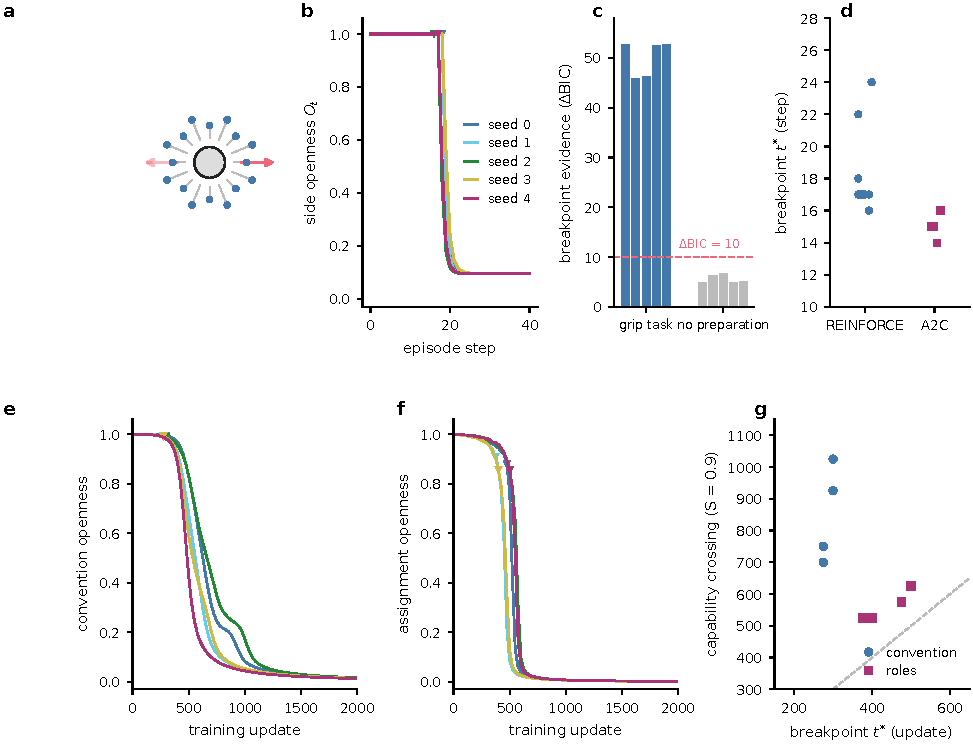
\includegraphics[width=\textwidth]{fig2.pdf}
\caption{\textbf{Punctuated realization in a learned collective.}
\textbf{a},~The grip-then-push transport task ($N=16$): agents must jointly
grip before the object can be pushed (arrows, the two possible push
directions), structurally delaying the choice of side.
\textbf{b},~Side-openness of the joint policy holds on a plateau and then
collapses; triangles mark the fitted breakpoint $t^{*}$ (5 REINFORCE
seeds).
\textbf{c},~Mechanism contrast: the grip task shows a breakpoint in 5/5
seeds ($\Delta$BIC well above 10) whereas a matched no-preparation task
shows none (0/5).
\textbf{d},~Breakpoint location across seeds and algorithms: 10/10 for
REINFORCE, and a strong partial replication under A2C (5/5 shape and
primary hinge, 3/5 strict).
\textbf{e},~Non-constructed positive I: a ten-agent signalling
population with 120 exactly equivalent codes and no gate holds a flat
open plateau, then commits with an onset breakpoint (4/5 seeds;
triangles), each seed to a different code.
\textbf{f},~Non-constructed positive II: six agents locking into a
division of labour among 720 equivalent role permutations (5/5 onset,
five distinct permutations).
\textbf{g},~In all nine onset seeds the possibility-space breakpoint
precedes the capability crossing ($S=0.9$): commitment is measurable
before the ability is expressed.}
\end{figure}

\begin{figure}[t]
\centering
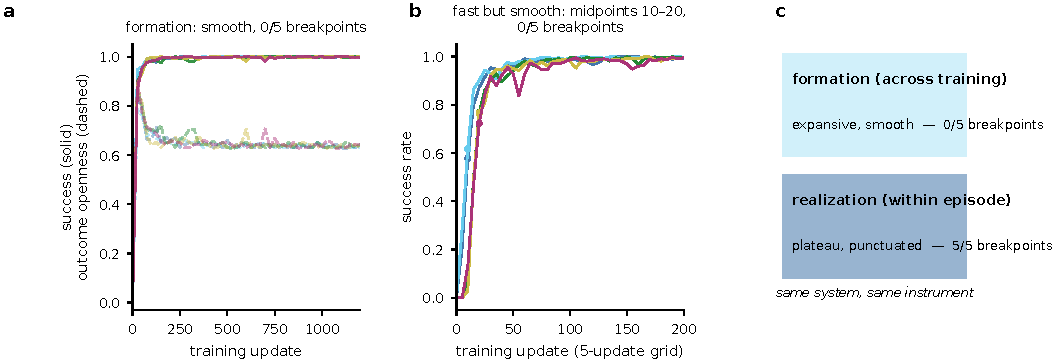
\includegraphics[width=0.78\textwidth]{fig3.pdf}
\caption{\textbf{Two timescales dissociate in one learned system.}
\textbf{a},~Formation axis (across training): success (solid) and outcome
openness (dashed) rise smoothly, no breakpoint (0/5).
\textbf{b},~At fine 5-update resolution the success rise is fast (per-seed
midpoints, dots, at updates 10--20) but still has no structural onset
(0/5). Formation is smooth and expansive while realization within an
episode is punctuated (Fig.~2b)---same system, same instrument.}
\end{figure}

\begin{figure}[t]
\centering
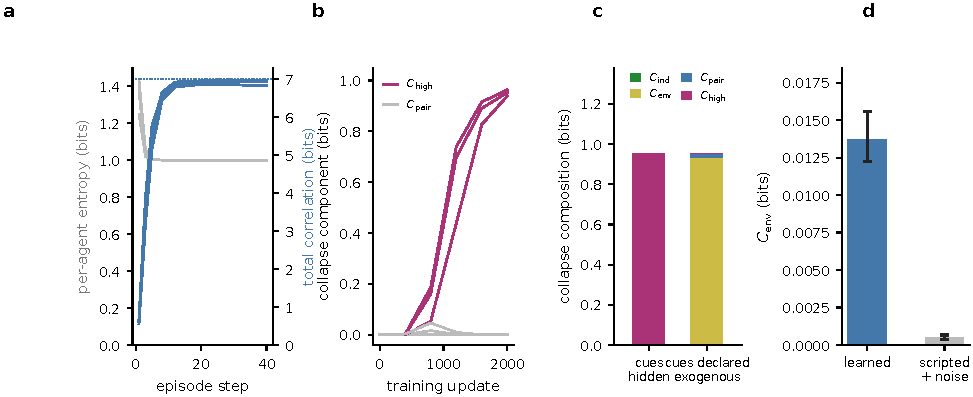
\includegraphics[width=\textwidth]{fig4.pdf}
\caption{\textbf{The source typology transfers to learning.}
\textbf{a},~Hidden-coordination task: per-agent entropy stays open while
total correlation rises to near the 7-bit maximum---a purely relational
collapse.
\textbf{b},~With the low-order route blocked, learning builds an
irreducible higher-order (XOR) carrier: $C_\mathrm{high}$ grows while
$C_\mathrm{pair}$ stays near zero.
\textbf{c},~Contract-relativity on the learned system: declaring the
private cues exogenous re-attributes the identical collapse from
$C_\mathrm{high}$ to $C_\mathrm{env}$.
\textbf{d},~At matched task score, the environment-conditioned component
separates a learned pair from a noise-matched scripted pair
(non-overlapping 95\% confidence intervals).}
\end{figure}

\begin{figure}[t]
\centering
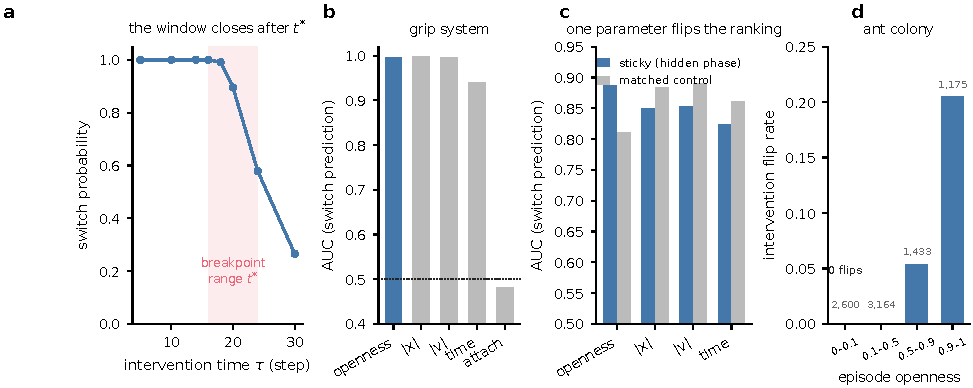
\includegraphics[width=\textwidth]{fig5.pdf}
\caption{\textbf{Remaining openness predicts controllability.}
\textbf{a},~Grip system: probability that a counter-regime impulse switches
the outcome, as a function of intervention time; the window closes after
the breakpoint range (shaded).
\textbf{b},~Openness predicts switchability as well as or better than
physical baselines (AUC).
\textbf{c},~Matched-parameter causal contrast: openness beats the order
parameter only when a hidden consolidation phase exists (sticky), and the
ranking reverses in the control.
\textbf{d},~Ant colony, paired counterfactuals: intervention flip-rate
rises with the episode's own remaining openness; closed episodes never
flip.}
\end{figure}

\begin{figure}[t]
\centering
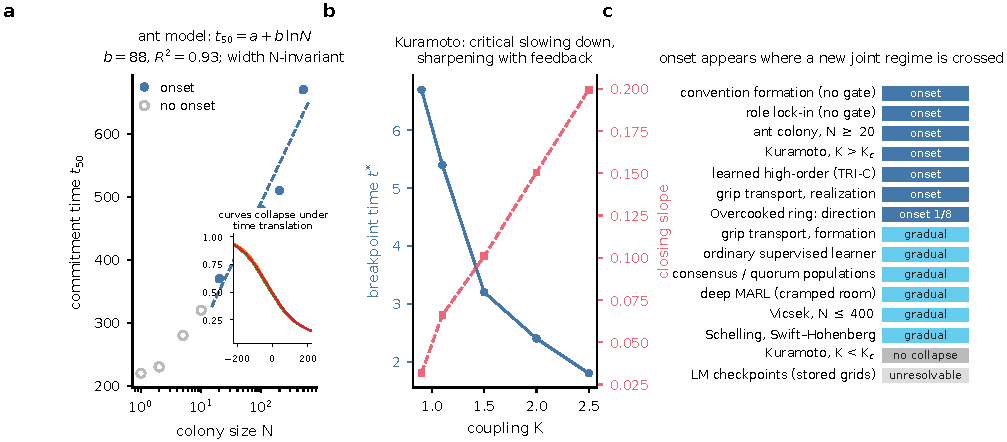
\includegraphics[width=\textwidth]{fig6.pdf}
\caption{\textbf{Scaling and scope.}
\textbf{a},~Finite-size scaling in the ant model: commitment time is
consistent with $t_{50}=a+b\ln N$ ($b=88$, 95\% CI [41, 124],
$R^{2}=0.93$; dashed
fit), as predicted by nucleation from $N^{-1/2}$ fluctuations; open
circles, sizes below the onset threshold (see Extended Data Fig.~2
for the universal collapse profile).
\textbf{b},~Kuramoto criticality: breakpoint time falls and closing slope
rises as coupling increases; subcritical runs are gated null.
\textbf{c},~Classification: onset appears where a joint-regime barrier
is crossed---including without any designed gate (convention formation,
role lock-in) and in the standard Overcooked coordination-ring layout,
where all 8 seeds commit to a circulation direction and 1/8 certifies
onset (Results)---and is absent for gradual convergence (formation,
ordinary learners, consensus/quorum populations, cramped-room deep
MARL, several classic cases).}
\end{figure}

\clearpage
\setcounter{figure}{0}
\renewcommand{\figurename}{Extended Data Fig.}

\begin{figure}[p]
\centering
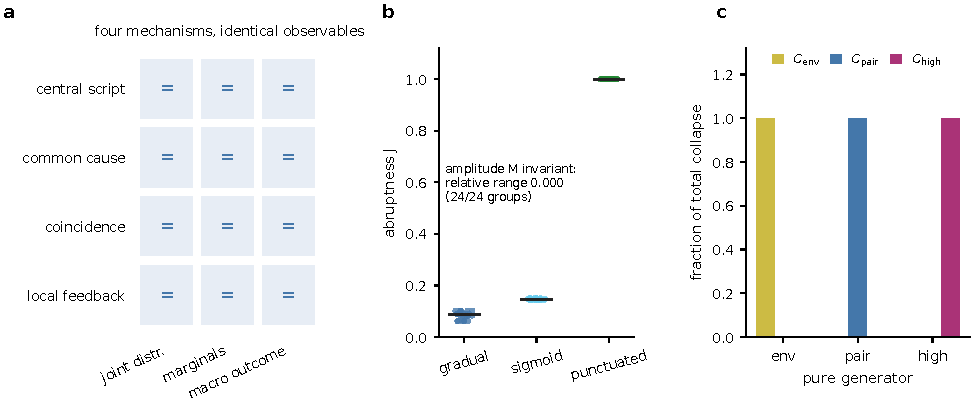
\includegraphics[width=0.72\textwidth]{edfig1_instrument.pdf}
\caption{\textbf{Instrument validation on constructed ground truth.}
\textbf{a},~Source-decomposition ladder on analytic ground truth: each pure
generator loads almost entirely onto its own component.
\textbf{b},~Full-factorial calibration (72 cells): amplitude $M$ is
invariant across temporal shape while abruptness $J$ strictly orders
punctuated $>$ sigmoid $>$ gradual.}
\end{figure}

\begin{figure}[p]
\centering
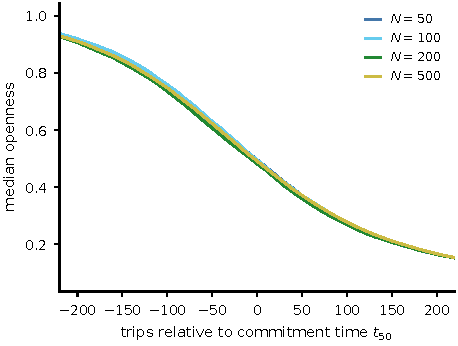
\includegraphics[width=0.55\textwidth]{edfig2_fss_collapse.pdf}
\caption{\textbf{Finite-size universality of the collapse profile.}
Median openness trajectories for ant colonies of $N=50$--$500$,
aligned by commitment time $t_{50}$: the four profiles superpose under
pure time translation (mean pairwise RMS 0.010 versus 0.266
unaligned). Increasing $N$ shifts the timing but does not reshape the
collapse.}
\end{figure}

\end{document}
